\documentclass[SSS_Laborbericht.tex]{subfiles}
\usepackage{pdfpages}
\usepackage{listings}

\begin{document}

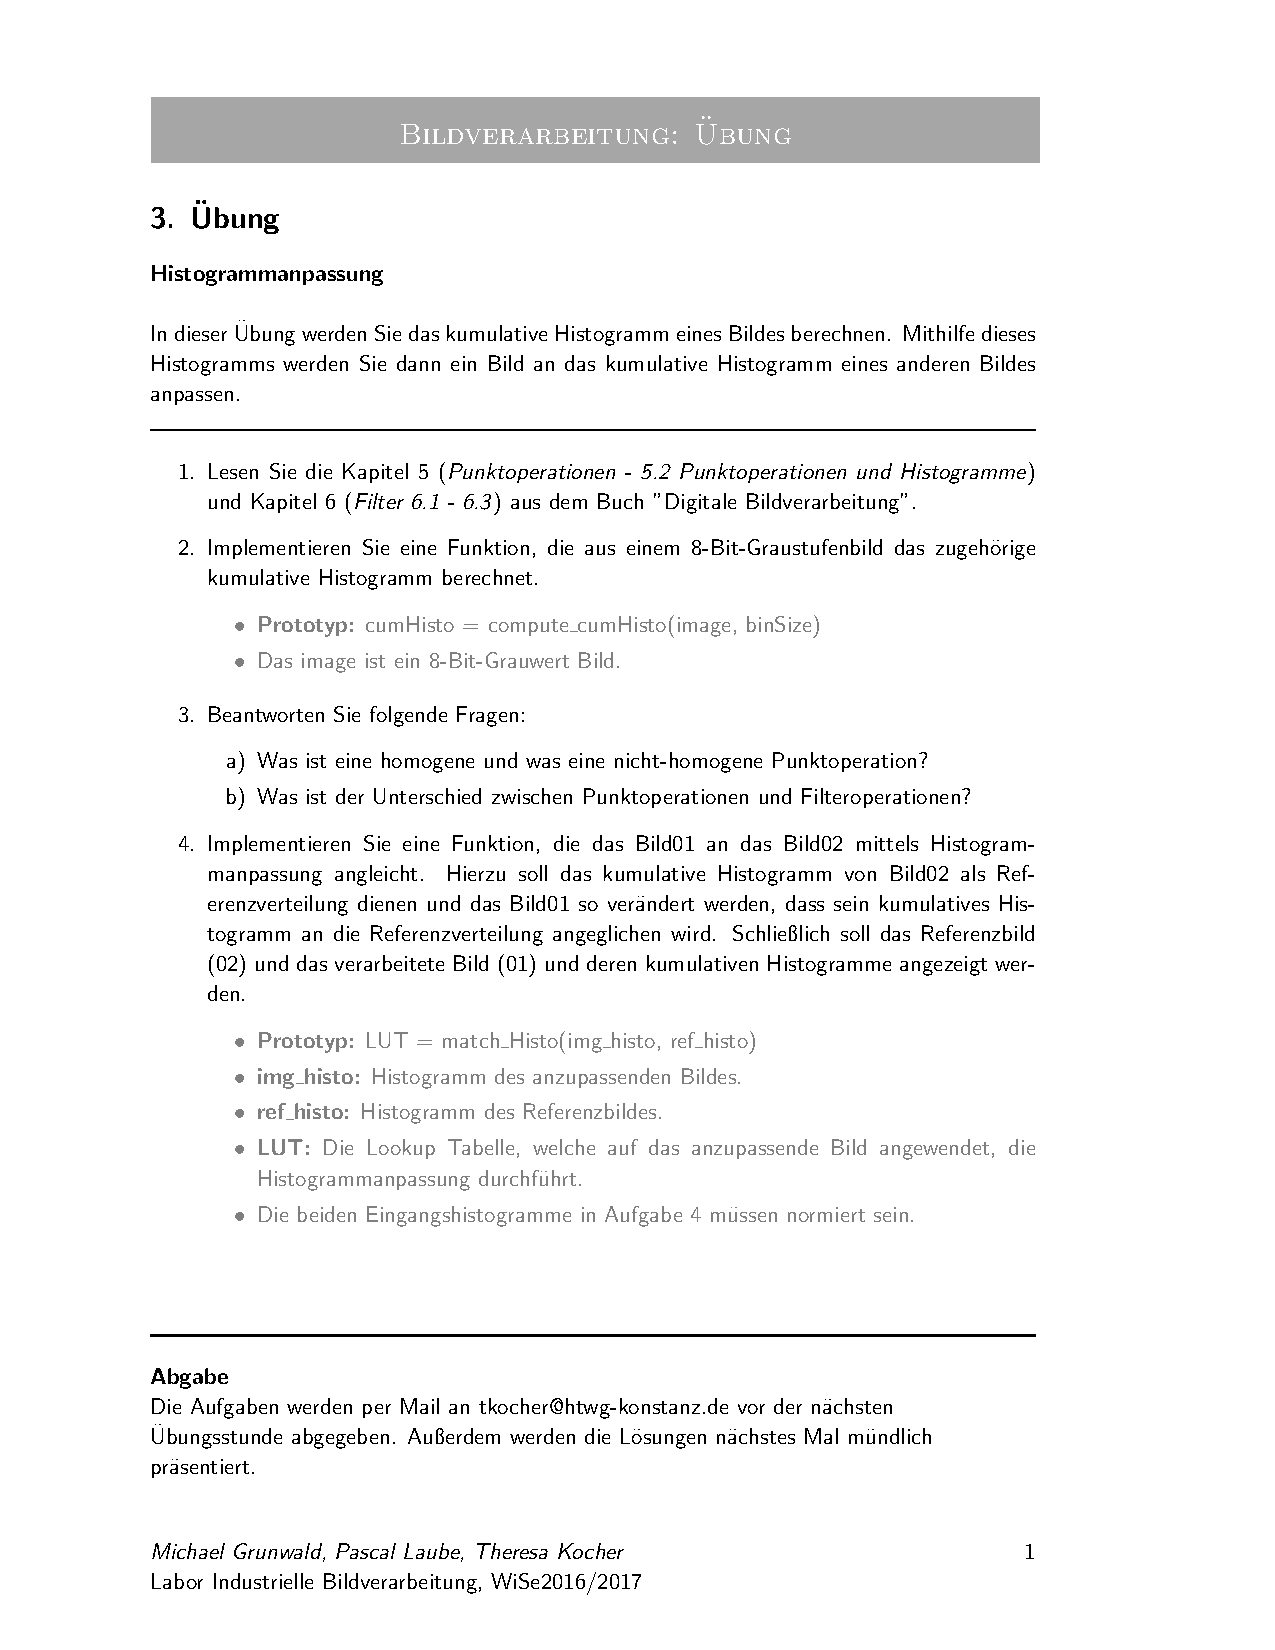
\includepdf[pages={1}]{uebung3.pdf}

\noindent\Large{Aufgabe 2}
\lstinputlisting[style=PYTHON, frame=single, caption=compute_cumHisto, firstline=7, lastline=11, firstnumber=7]{template.py}

\noindent\Large{Aufgabe 3 Code}
\lstinputlisting[style=PYTHON, frame=single, caption=matchHisto, firstline=24, lastline=38, firstnumber=24]{template.py}

\noindent\Large{Aufgabe 3 Code}
\lstinputlisting[style=PYTHON, frame=single, caption=matchHisto, firstline=60, lastline=77, firstnumber=24]{template.py}

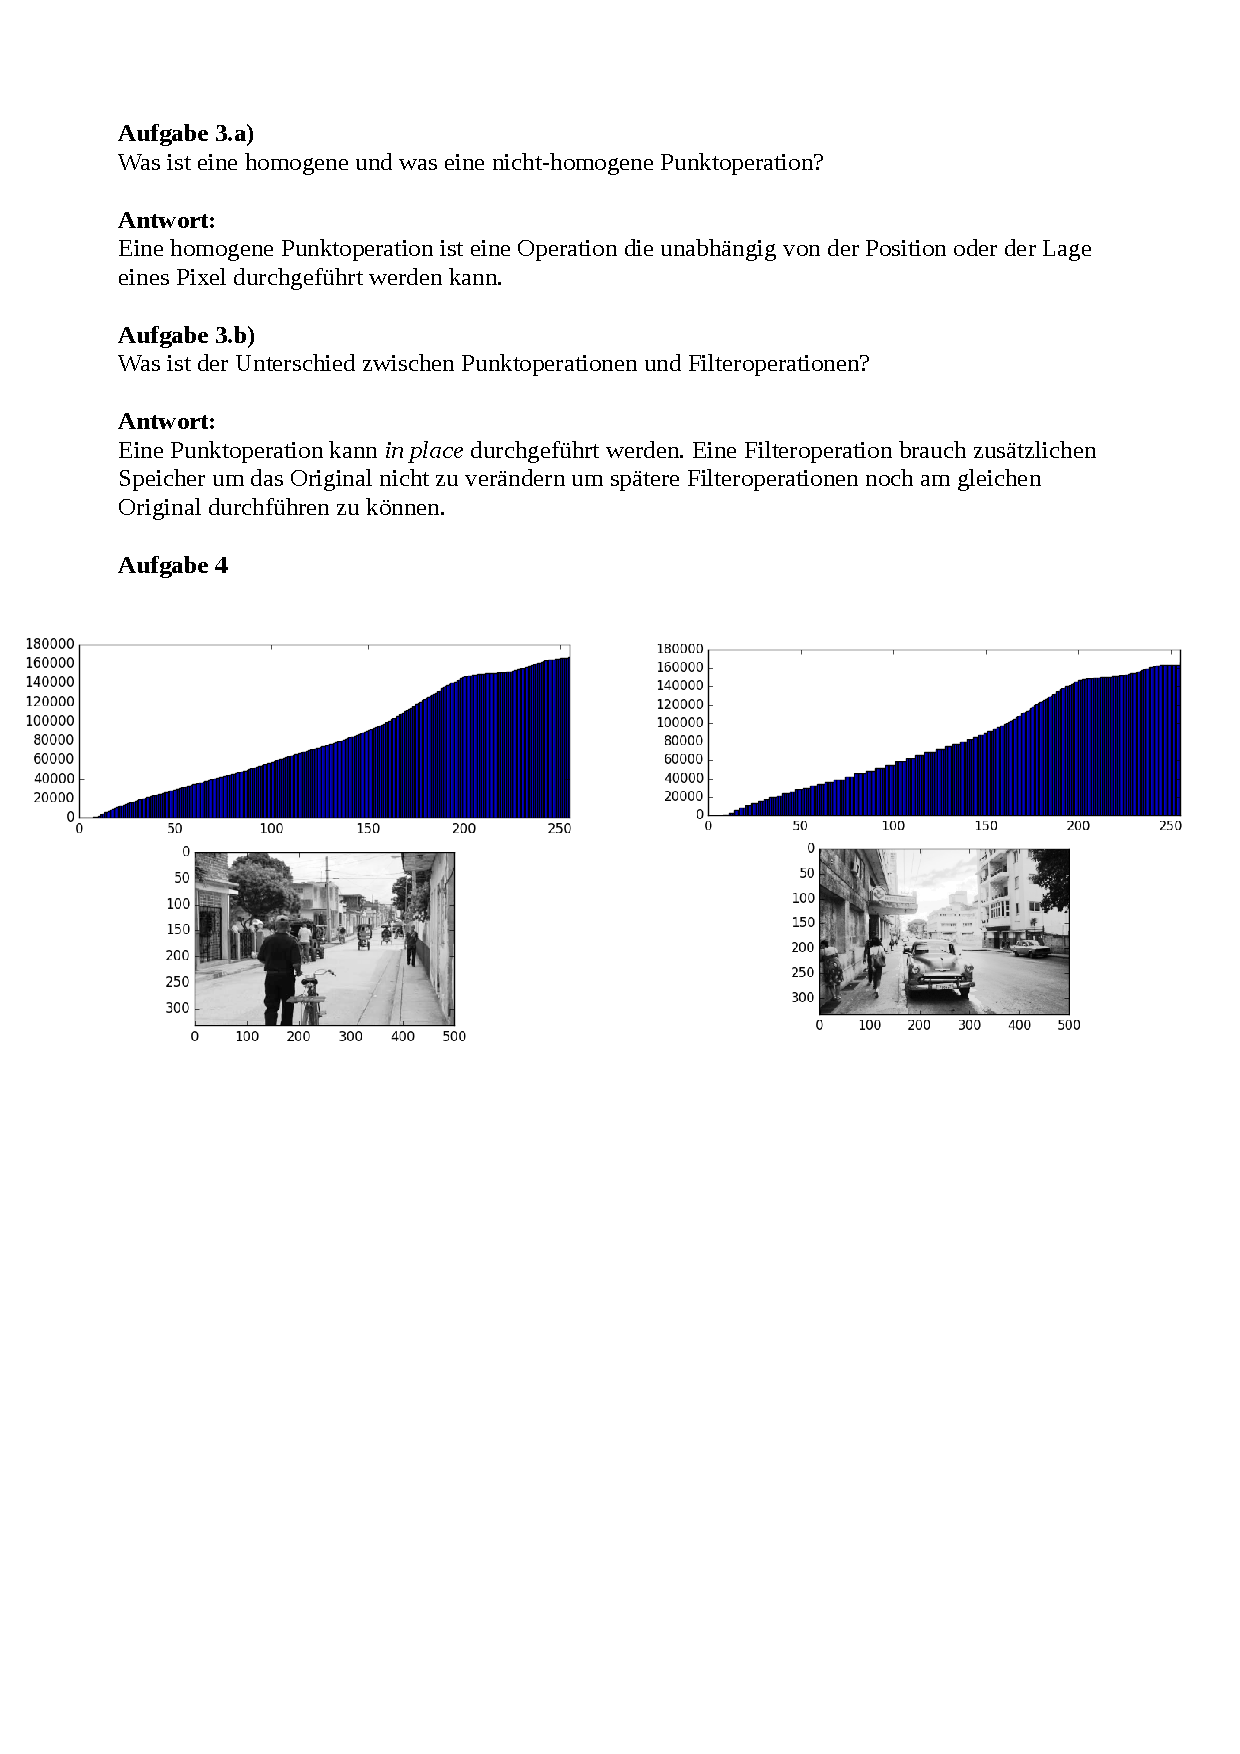
\includepdf[pages={1}]{Aufgabe3und4.pdf}

\end{document}